\documentclass[a4paper, 10pt, twocolumn]{article}

% Configuration {{{
\usepackage[utf8]{inputenc}
\usepackage[T2A]{fontenc} % T1 for English
\usepackage[english, russian]{babel}

\usepackage{enumitem}
\setlist{nolistsep}
\usepackage{mathtools}
\usepackage{xcolor}
\definecolor{dimblue}{HTML}{1010aa}
\usepackage[
	colorlinks=true, 
	allcolors=dimblue
]{hyperref}
\usepackage[
	vmargin=1in,
	hmargin=.8in
]{geometry}
\setlength{\columnsep}{.25in}
%\usepackage[nospread]{flushend}
\usepackage{cuted}
\linespread{1.3}
\usepackage{indentfirst}
\usepackage{graphicx}
\usepackage{tikz}
\usepackage[multidot]{grffile}
\usepackage[labelsep=period]{caption}
\usepackage{subcaption}
\usepackage{multirow}

\usepackage{titlesec}
\titleformat{\section}[hang]{\bf\centering}{\thesection.}{.5em}{}[]
\def\thesection{\Roman{section}}
\def\thefootnote{\fnsymbol{footnote}}

%\usepackage{times} % for English

\def\eps{\varepsilon}
\def\avg#1{\left\langle#1\right\rangle}
\def\H{\mathcal{H}}
\let\ophi\phi
\let\phi\varphi
% }}}

\begin{document}

% Title {{{
\begin{strip}
\begin{center}
\vskip-2.4\baselineskip
{\large\textbf{Наклонная ось вращения в ротационных возбуждениях атомных ядер}}
\vskip.3\baselineskip
{Керим Гусейнов\footnotemark}
\vskip.0\baselineskip
\textit{МГУ им. М. В. Ломоносова, кафедра общей ядерной физики}
\vskip.3\baselineskip
\today
\end{center}
\end{strip}
\footnotetext{\href{mailto:guseynovkerim@gmail.com}{guseynovkerim@gmail.com}}
% }}}

\section{Введение}% {{{

В университетских курсах наибольшее внимание уделяется сферическим ядрам 
ввиду наибольшей простоты аналитического рассмотрения. Следующими 
в очереди идут ядра, имеющие форму эллипсоида вращения, то есть 
двухосного эллипсоида. Несмотря на то, что большинство ядер в основном 
состоянии действительно имеет сферическую или хотя бы осевую симметрию, 
нет причин полагать, что этими формами исчерпывается все разнообразие 
ядер. Напротив, многочисленные исследования показали, что даже 
в основном состоянии многие ядра не имеют осевой 
симметрии~\cite{gs1,gs2,gs3}. Среди таких форм самой очевидной является 
трехосный эллипсоид, который будет подробно рассмотрен далее.

Наличие трех разных осей приводит к многим изменениям свойств ядра, 
включая энергии отделения нуклонов, высоту барьера деления, фрагментацию 
состояний с коллективными возбуждениями большой амплитуды и вероятность 
испускания протона. Однако, задача прямого измерения трехосности до сих 
пор является очень сложной. Поэтому немалые усилия прилагаются для 
поиска явных сигнатур трехосности, таких как инверсия энергетических 
уровней наинизшей квазичастицы с большим моментом $j$ и чередование 
$\gamma$-серий. Последнее уже применяется для идентификации жесткой 
и динамической трехосности и использовалось для выдвижения 
соответствующих кандидатов ядер~\cite{gamma-rigid}.
Кроме того, существуют явления, появляющиеся исключительно в трехосных 
ядрах. Среди них можно назвать нарушение хиральной симметрии 
и качающиеся (wobbling) возбуждения. Последние позволили доказать 
отсутствие аксиальной симметрии в ядрах $^{161,163,165,167}$Lu, а также 
$^{167}$Ta и $^{135}$Pr. Все эти ядра, очевидно, нечетные, и считается, 
что в них такая форма обусловлена, помимо остаточного взаимодействия, 
поведением неспаренного нуклона и его взаимодействием с квазичастицами 
кора ядра.

Менее популярным, но не менее занимательным эффектом является вращение 
ядра вокруг оси, наклоненной относительно собственных осей эллипсоида 
инерции. Такое поведение не было идентифицировано во многих изотопах, во 
всяком случае до сих пор, но представляет большой интерес для понимания 
вращательных степеней свободы в ядрах.

% }}}

\section{Общий случай трехосного ротора}% {{{

Трехосный эллипсоид определяется поверхностью
$$ R(\theta, \phi) = R_0 \left(1 + a_0 Y_{20} + a_2(Y_{22} + Y_{2-2})\right), $$
$$ a_0 = \beta\cos\gamma, \quad a_2 = \frac{\beta}{\sqrt{2}}\sin\gamma, \quad \gamma \in \left[0, \frac{\pi}{3}\right]. $$

Впервые жесткий трехосный ротор был использован в ядерной физике нашими 
соотечественниками Давыдовым и Филипповым~\cite{first-use}, которые 
показали, что низколежащие коллективные возбуждения в некоторых ядрах 
можно описать собственными значениями гамильтониана ротора с разными 
моментами инерции вдоль осей собственной системы отсчета.

С тех пор теоретики вели активные поиски ядер, в которых может 
наблюдаться наличие трех разных осей. Например, в~\cite{gs3} было 
модельно рассмотрено порядка 8 тысяч ядер и было найдено, что несколько 
сотен из них имеют значение $\gamma$, не равное $0$ или $\pi/3$ даже 
в основном состоянии. Наибольшее влияние аксиальной асимметрии 
наблюдалось для ядер вблизи $^{108}$Ru. На 
рисунке~\ref{fig:delta-e-gamma} представлена $N-Z$ диаграмма ядер 
с наибольшим значением коррекции энергии основного состояния при 
вариации параметра $\gamma$
$$\Delta E_\gamma = \min_{\eps_2,\eps_4} E(\eps_2, \eps_4, \gamma=0)
  - \min_{\eps_2, \eps_4, \gamma} E(\eps_2, \eps_4, \gamma).$$
Как видно, имеется несколько областей, в которых значение $\gamma$ 
нетривиально.

\begin{figure}% {{{
	\centering
	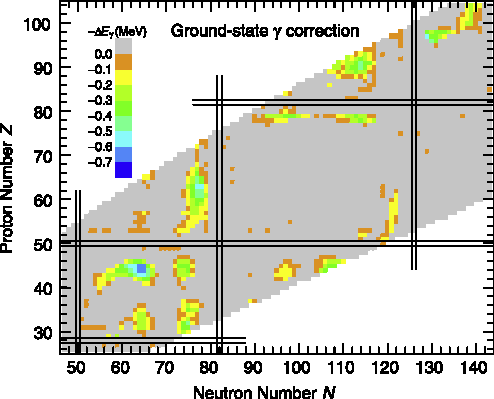
\includegraphics[width=\linewidth]{figures/delta-e-gamma}
	\caption{$N-Z$ диаграмма ядер с наибольшим значением коррекции энергии основного состояния при учете параметра $\gamma$.}
	\label{fig:delta-e-gamma}
\end{figure}% }}}

Перейдем теперь к изучению трехосного ротора. Поскольку конечной целью 
является описание вращения вокруг наклонной оси, то есть оси, не 
перпендикулярной ни одной из главных осей эллипсоида, необходимо сразу 
перейти к общему случаю. Наиболее общий квадратичный по угловому моменту 
гамильтониан имеет вид
$$ H = A_1 J_1^2 + A_2 J_2^2 + A_3 J_3^2 + B_1 J_1 + B_2 J_2 + B_3 J_3. $$
Даже в этом случае $[H, J^2] = 0$, а значит
$$ J_1^2 + J_2^2 + J_3^2 = J^2 = j(j+1). $$
Без ограничения общности перепишем гамильтониан в виде
$$ H = (A_1 - A_2) (J_1^2 + u J_2^2 + 2 v_0 J_3) + A_3 J^2, $$
$$ u = \frac{A_2 - A_3}{A_1 - A_2}, \ 
	 v_0 = \frac{B}{2(A_1 - A_2)}, \ 
	 u \in [-1, 1],\ v \geq 0. $$
Решить эту задачу удобнее всего с помощью полуклассического 
вариационного подхода. Для этого рассматривается вариация
$$ \delta \int \langle \psi(z) | H - \partial_t | \psi(z) \rangle d t = 0, $$
где $z$ -- комплексная переменная, зависящая от времени, а для волновой 
функции выбирается форма
$$|\psi(z)\rangle = N e^{z J_-} |J, J\rangle. $$
Используя соотношения
$$ \avg{J_3} = J - \frac{2Jzz^*}{1 + zz^*},$$
$$ \avg{J_1^2} = \frac{1}{4}\left(2J + \frac{2J (2J - 1)}{(1 + zz^*)^2}
   (z + z^*)^2\right), $$
$$ \avg{J_2^2} = -\frac{1}{4}\left(-2J + \frac{2J (2J - 1)}{(1 + zz^*)^2}
   (z - z^*)^2\right), $$
$$ \avg{J_3^2} = J^2 - \frac{2J (2J - 1)zz^*}{(1 + zz^*)^2}, $$
$$ \avg{\partial_t} = \frac{J (\dot zz^* - z\dot z^*)}{1 + zz^*}, $$
переходим к гамильтониану как функции независимых переменных $z$, $z^*$, 
обозначаем $\avg{H} = \H$ и получаем
$$ \frac{\partial \H}{\partial z} = - \frac{2iJ\dot z^*}{(1 + zz^*)^2},\quad
   \frac{\partial \H}{\partial z^*} =  \frac{2iJ\dot z}{(1 + zz^*)^2}. $$
Удобно ввести новые переменные
$$ r = \frac{2J}{1 + zz^*}, \quad \phi = \mathrm{arg}\,z, $$
в которых предыдущие уравнения выглядят как
$$ \frac{\partial \H}{\partial r} = \dot \phi,\quad
   \frac{\partial \H}{\partial \phi} =  - \dot r. $$
Таким образом, введенные переменные $r$, $\phi$ канонически сопряжены. 
Рассмотрим также переменные $\xi = \avg{J_3} = r - J$, $\ophi = - \phi$, 
в которых уравнения принимают вид
$$ \frac{\partial \H}{\partial \xi} = - \dot \ophi,\quad
   \frac{\partial \H}{\partial \ophi} =  \dot \xi, $$
а значит, они тоже сопряжены. $\xi$ при этом выступает в роли 
координаты, а $\ophi$ -- импульса.

Для описания полного гамильтониана удобно сначала рассмотреть часть 
в скобках отдельно
$$ h = J_1^2 + u J_2^2 + 2 v_0 J_3. $$
Проводя для него процедуру перехода к классике $ h = x_1^2 + u x_2^2 
+ 2 v x_3$,  при которой
$$ \{x_i, x_j\} = \eps_{ijk} x_k, $$
получаем $\dot x_i = \{x_i, h\}$, поскольку, как было видно выше, $x_3, 
\ophi$ -- канонические переменные. Тогда
$$ \dot x_1 = 2 x_2 (u x_3 - v),\;\:
   \dot x_2 = 2 x_1 (x_3 - v), \;\:
	 \dot x_3 = 2(1 - u) x_1 x_2. $$
Отсюда видно, что $\dot h = 0$, а значит, это интеграл движения, и его 
можно по праву обозначать $E$. Траектории в пространстве $x_1,\ x_2,\ 
x_3$, таким образом, определяются пересечением поверхностей $x_1^2 
+ x_2^2 + x_3^2 = 1$ и $x_1^2 + u x_2^2 + 2v x_3 = E = \mathrm{const}.$

При дальнейшем поиске стационарных точек, для которых $\partial 
E / \partial x_i = 0$, необходимо заметить, что интерес также 
представляют вырожденные точки, в которых
$$ \mathrm{det} \left| \frac{\partial^2 E}{\partial x_i \partial x_j} \right| = 0. $$
Последнее уравнение эквивалентно
$$ f(u,v) = (1-u)(1-v)(u^2 - v^2) = 0 $$
и описывает сепаратрисы.
В таблице~\ref{tab:crit} приведены стационарные точки, энергии в них, 
а также ограничения на $u,\ v$, необходимые для реализации точек. На 
рисунке~\ref{fig:crit-e} показано, как ведут себя критические энергии 
в зависимости от параметров модели. На рисунке~\ref{fig:traj} показаны 
поверхности, соответствующие классическим траекториям движения вблизи 
стационарных точек. Максимумы и минимумы окружены замкнутыми 
непересекающимися траекториями, которые отделены сепаратрисами от 
траекторий, замкнутых вокруг других экстремумов.

\begin{table*}% {{{
	\centering
	\caption{Классические стационарные точки гамильтониана $ h = x_1^2 
	+ u x_2^2 + 2 v x_3$, их энергии и соответствующие ограничения на 
	параметры гамильтониана. В последнем столбце указан тип точки: M -- 
	максимум, m -- минимум, s -- седло.}
	\label{tab:crit}
	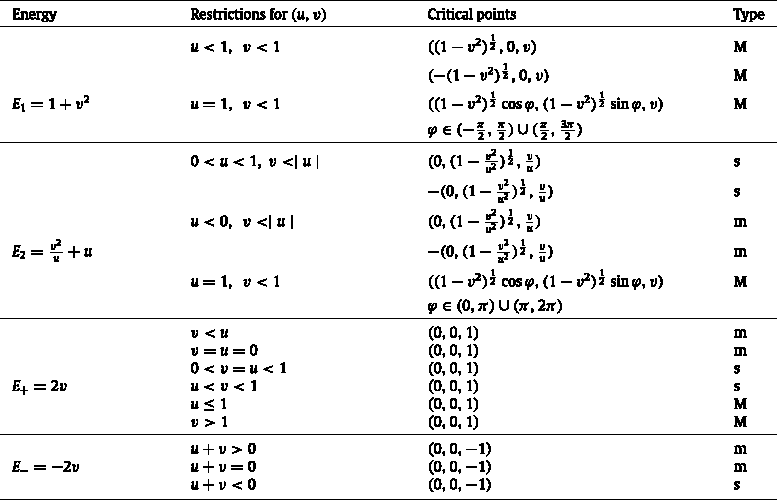
\includegraphics[width=.7\linewidth]{figures/crit-table}
\end{table*}% }}}

\begin{figure}% {{{
	\centering
	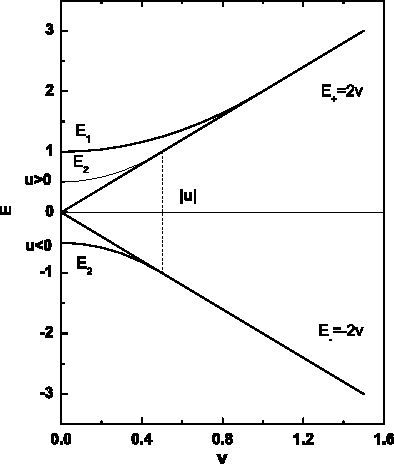
\includegraphics[width=.7\linewidth]{figures/crit-energy}
	\caption{Поведение критических энергий гамильтониана $ h = x_1^2 
	+ u x_2^2 + 2 v x_3$ в зависимости от параметра $v$ при фиксированном 
	значении $u$.}
	\label{fig:crit-e}
\end{figure}% }}}

\begin{figure}% {{{
	\centering
	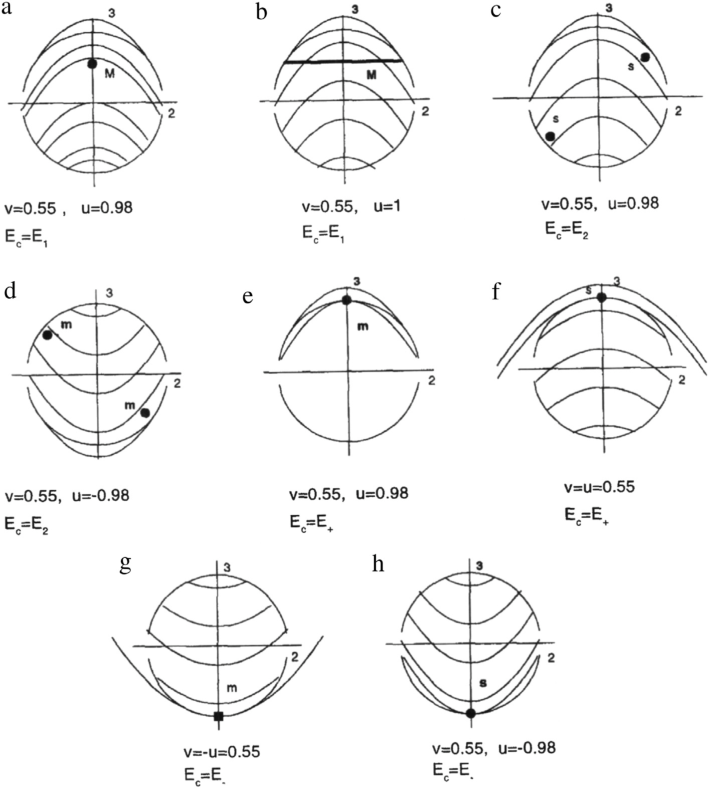
\includegraphics[width=\linewidth]{figures/trajectories}
	\caption{Сечение поверхностей $ x_1^2 + u x_2^2 + 2 v x_3 = E $ и $x_1^2 + x_2^2 + x_3^2 = 1$ с плоскостью $x_1 = 0$ вблизи критических точек.}
	\label{fig:traj}
\end{figure}% }}}

Можно заключить, что, во-первых, для определенных областей пространства 
параметров $(u,v)$ критические точки окружены периодическими 
траекториями, и периоды испытывают разрыв при пересечении сепаратрис. 
Во-вторых, вблизи седловых точек некорректно линейно раскладывать 
гамильтониан, поскольку он нестабилен относительно одной из координат. 
В-третьих, периоды траекторий для $E_+ = 2v$ при $v < u < 1$ и для $E_2 
= v^2/u + u$ при $u < v$, $u \in [0, 1)$ в точности совпадают 
с результатами линеаризации.

Учитывая, что ограничения для реализации критических точек оставляют 
лишь одну свободную переменную, для нахождения периодов необходимо взять 
интеграл
$$ t \!-\! t_0 =\! \int_{x_{30}}^{x_3} \frac{dx}{2\sqrt{|u| (x \!-\! \alpha_1) (x \!-\! \alpha_2) (x \!-\! \alpha_3) (x \!-\! \alpha_4)}}, $$
где $\alpha_1 = v - \sqrt{E_1 - E}$, $\alpha_2 = v + \sqrt{E_1 - E}$,
$\alpha_3 = v/u - \sqrt{(E_2 - E)/u}$, $\alpha_4 = v/u + \sqrt{(E_2 - E)/u}$.
Период, таким образом, выражается через гипергеометрическую функцию.

Для последнего этапа, квантования, применяется правило Бора 
и Зоммерфельда
$$ S = \int_{E_0}^E T(E') d E' = 2\pi \hbar n, $$
где $E_0$ -- энергия ближайшего экстремума. Исходя из формальных равенств,
$$ \frac{\partial S}{\partial E} = T(E) = \frac{\partial S}{\partial n}
   \frac{\partial n}{\partial E}\ \Rightarrow\ \frac{\partial E}{\partial n} =
	 \frac{2\pi\hbar}{T(E)}. $$
Таким образом, мы получили дифференциальное уравнение, из которого можно 
найти энергию. Линейная зависимость энергии от $n$ получается лишь 
в случае, когда период не зависит от энергии, то есть при использовании 
нулевого приближения при разложении в точке $E_0$.

% }}}}

\section{Вращение вокруг наклонной оси}% {{{

Рассмотрим трехосный эллипсоид, который вращается так, что его угловой 
момент направлен вдоль оси $z$ лабораторной системы координат $(x,y,z)$. 
Собственную систему координат эллипсоида назовем $(1,2,3)$. Возможны 
следующие конфигурации.

(1) Ось $z$ совпадает с одной из собственных осей, например, 3. Тогда 
вращение на угол $\pi$ не приводит к изменению функции распределения 
плотности, а значит, возникает ограничение на изменение орбитального 
момента $J = \alpha + 2n$, $n \in Z_+$. Для заданного $\alpha$ возникает 
единая спектральная серия, характеризующаяся $\Delta l = 2$. Эта 
ситуация приведена на рисунке~\ref{fig:triax} сверху.

(2) Ось вращения лежит в одной из главных плоскостей, например, $(1,3)$. 
Тогда поворот $R_z$ на угол $\pi$ вокруг оси $z$ приводит к изменению 
плотности, как видно из центральной части рисунка~\ref{fig:triax}. 
В результате $\alpha$ перестает быть хорошим квантовым числом, 
а ограничение на орбитальный момент снимается. Такая вращательная серия 
имеет $\Delta l = 1$ и образована двумя разными вырожденными сериями, 
для которых $\Delta l = 2$. Хиральная симметрия $TR_y$ при этом 
сохраняется.

\begin{figure}[t]% {{{
	\centering
	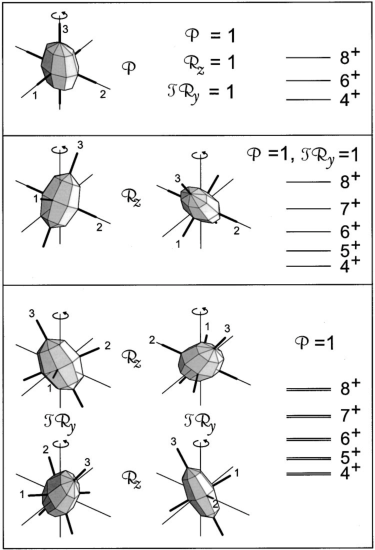
\includegraphics[width=.8\linewidth]{figures/triaxial-ellipsoid}
	\caption{Вращение трехосного эллипсоида вокруг одной из его осей 
	(сверху), вокруг оси, лежащей в одной из его главных плоскостей (по 
	центру), вокруг произвольной оси (снизу). На рисунке проиллюстрированы 
	дискретные симметрии: $P$ -- инверсия координат, $R_{y,z}$ -- поворот 
	на $\pi$ вокруг $y,z$, $T$ -- инверсия по времени.}
	\label{fig:triax}
\end{figure}% }}}

(3) Ось вращения не находится в какой-либо плоскости главных осей 
эллипсоида, то есть не перпендикулярна ни одной из последних. В этом 
случае операция $TR_y$ уже не сохраняет плотность распределения и даже 
меняет хиральность осей $(1,2,3)$ относительно $J$. Левые и правые 
системы координат соответствуют одинаковой энергии, следовательно, 
имеются две серии, для каждой из которых $\Delta l = 1$. Четыре 
вырожденных решения предсказываются как моделью вращения вокруг 
наклонной оси, так и частично-дырочной моделью. Эти решения можно 
получить путем отражения $J$ относительно плоскостей $(1,3)$ и $(2,3)$. 
Концы четырех изображений можно совместить для получения прямоугольника, 
в центре которого находится ось 3. Решения, находящиеся на концах каждой 
диагонали, можно получить друг из друга преобразованием $R_3$. Каждую 
пару таких состояний можно объединить в пару вырожденных состояний, 
формирующих серию $\Delta l = 1$. Так, две диагонали определяют две 
серии $\Delta l = 1$, отличающиеся хиральностью. Состояния этих серий 
отличаются преобразованием хиральности. При восстановлении хиральной 
симметрии путем подбора линейных комбинаций серии разъединяются. 
Расщепление серий аналогично расщеплению энергетических состояний 
асимметричных относительно инверсии координат систем.

Таким образом, хиральность присуща лишь ядрам, вращающимся вокруг 
наклонной оси. В отличие от молекулярной хиральности, которая статична, 
ядерная -- динамична, поскольку угловой момент задает направление, 
относительно которого определяется правость или левость системы 
$(1,2,3)$.

Движение вне основных плоскостей может возникать в одной протонной 
частице, одной нейтронной дырке и трехосном коре. Орбитальный момент 
протона располагается вдоль длинной оси (l), нейтрона -- вдоль короткой 
оси (s), а кор вращается вокруг оси с наибольшим моментом инерции, то 
есть промежуточной оси (i). В начале хиральных серий момент кора мал, 
и ось вращения лежит в плоскости $(s,l)$. По мере увеличения общего 
момента увеличивается и момент кора, что приводит в дальнейшем 
к переориентации момента частицы и дырки вдоль той же оси $i$, поскольку 
это минимизирует силу Кориолиса. Хиральная структура серий отражается 
в электромагнитных переходах: невырожденный дублет характеризуется 
сильными $M1$ и слабыми $E2$ переходами внутри серии. Скорости этих 
переходов уменьшаются по мере возрастания орбитального момента.

% }}}

\section{Случай нечетных ядер}% {{{

\def\Pr#1{$^{135}$Pr}

Изначально трехосные ядра было предложено искать среди четно-четных, 
однако долгие поиски таких не увенчались успехом, и стало понятно, что 
стоит обратить внимание к другим ядрам. Теоретически можно объяснить 
существование такой деформации в ядрах с одним неспаренным нуклоном или 
дыркой. В таком случае взаимодействие квазичастицы с кором в паре 
с ее плотностью распределения могут давать деформированное ядро. Как уже 
было сказано, трехосная деформация наблюдалась в четырех нечетных 
изотопах Lu, а также в $^{167}$Ta и $^{135}$Pr. При этом, только в \Pr{} 
наблюдалось окончание поперечных качающихся возбуждений~\cite{Pr1,Pr2}, 
что связывают с зависимостью условий их существования от величины 
орбитального момента. Достижение соответствующего предела приводит 
к возникновению вращения вокруг наклонной оси. Таким образом, есть смысл 
рассмотреть условия, при которых происходит поперечная мода качения, 
а также переход к наклонной оси.

Поскольку мы имеем дело с нечетным ядром, удобно разделить гамильтониан 
на гамильтониан самог\'{о} трехосного ротора и гамильтониан неспаренной 
частицы
$$ H = H_R + H_\mathrm{sp}, $$
где $H_R = \sum_i A_i (J_i - j_i)^2$, $J$ -- момент всей системы, $A_i 
= 1/2\mathcal{J}_i$ -- моменты инерции ротора, а $j$ -- момент 
неспаренного нуклона. Вторая часть гамильтониана
$$\begin{aligned}
	H_\mathrm{sp} = \frac{V}{j(j+1)} \Big(&\big(3j_3^2 - j(j+1)\big) \cos \gamma - \\
	& - \sqrt{3} (j_1^2 - j_2^2) \sin \gamma \Big),
\end{aligned}$$
где $\gamma$ -- параметр асимметрии, который также определяет 
соотношение между $A_i$. Для упрощения рассмотрим случай, когда момент 
частицы расположен вдоль оси 1, $j_1 \approx j$, тогда
$$ H = A_1 (J_1 - j)^2 + A_2 J_2^2 + A_3 J_3^2 + \mathrm{const}, $$
что эквивалентно
$$ H = A_1 J_1^2 + A_2 J_2^2 + A_3 J_3^2 - 2 A_1 j J_1. $$
Применим такой же полуклассический подход, как был использован ранее, 
$|\psi(z)\rangle = N e^{zJ_-}|J, J\rangle$. Обозначая $z 
= \tg\frac{\theta}{2} \, e^{i\phi}$ и вводя $r = 2I \cos 
\frac{\theta}{2}$, получаем уравнения Гамильтона
$$ \frac{\partial H}{\partial r} = \dot \phi, \quad
   \frac{\partial H}{\partial \phi} = - \dot r. $$
Классический гамильтониан в этих переменных имеет вид
$$\begin{aligned}
	H(r, \phi) =&\ \frac{J}{2} (A_1 + A_2) + A_3 J^2 + \frac{(2J \!-\! 1) r (2J \!-\! r)}{2J}\!\times \\
	& \times (A_1 \cos^2\phi + A_2\sin^2\phi - A_3) - \\
	& - 2 A_1 j \sqrt{r(2J - r)} \cos\phi
\end{aligned}$$
при условии $J_1^2 + J_2^2 + J_3^2 = J^2$.

Эта система имеет три стационарные точки: $(r_1 = J, \phi_1 = 0)$,
$(\sqrt{r_2(2J - r_2)} = J, \phi_2 = \alpha_2)$
и $(\sqrt{r_3(2J-r_3)} = J\cos\alpha_3, \phi_3 = 0)$, где
$$\cos\alpha_{2,3} = \frac{2A_1j}{(2J-1)(A_1 - A_{2,3})}.$$
Условия, при которых эти точки являются минимумами, имеют вид:
\def\SJj{S_{Jj}}
\\ (1) $\SJj A_1 < A_2 < A_3$ или $\SJj A_1 < A_3 < A_2$,
\\ (2) $A_2 < A_3 < \SJj A_1$ или $A_2 < \SJj A_1 < A_3$,
\\ (3) $A_3 < A_2 < \SJj A_1$ или $A_3 < \SJj A_1 < A_2$,
где
$$ \SJj = \frac{2J - 1 - 2j}{2J - 1}.$$

Для получения энергетических уровней можно разложить гамильтониан вблизи 
каждой из этих точек и записать соответствующую энергию гармонического 
осциллятора. В результате получаются уровни
$$\begin{aligned}
	E_i(J, n) =& A_i J^2 + \frac{J}{2}\sum_{k\neq i} A_k - 2A_i jJ \cos\alpha_i + \\
	& + \omega_i(J) (n + 1/2),
\end{aligned}$$
где $\cos\alpha_1$ следует считать равным единице. Выражения для частот 
имеют вид
$$\begin{aligned}
	\omega_1(J) =&\ \sqrt{(2J - 1)(A_3 - A_1) + 2A_1j}\ \times \\
	& \times \sqrt{(2J - 1)(A_2 - A_1) + 2A_1 j},
\end{aligned}$$
$$ \omega_2(J) = (2J-1)\sqrt{(A_3 - A_2)(A_1 - A_2)}\sin\alpha_2, $$
$$ \omega_3(J) = (2J-1)\sqrt{(A_2 - A_3)(A_1 - A_3)}\sin\alpha_3. $$

В выражениях для энергий квадратичный по $J$ член соответствует обычному 
вращению, а линейный -- прецессии. Спектры $E_{2,3}$ соответствуют 
обычной качающейся моде, рассмотренной еще Бором и Моттельсоном, но 
наклоненной на угол $\alpha_{2,3}$ относительно исходной оси 1.

Далее, рассмотрим фазовую диаграмму, показывающую область доступных мод 
качения. Она представлена на рисунке~\ref{fig:independent} для 
независимых жестких моментов инерции и на рисунке~\ref{fig:hydrodyn} для 
гидродинамической модели. Независимо от модели, при увеличении 
орбитального момента возрастает величина $\SJj$ и приближается 
к единице, ограничивая область перпендикулярной моды качений. В конце 
концов, наступает момент, когда положение ядра на диаграмме оказывается 
внутри какой-либо из областей (2) и (3). Это будет означать переход 
к вращению с качением вокруг наклонной оси.

\begin{figure}% {{{
	\centering
	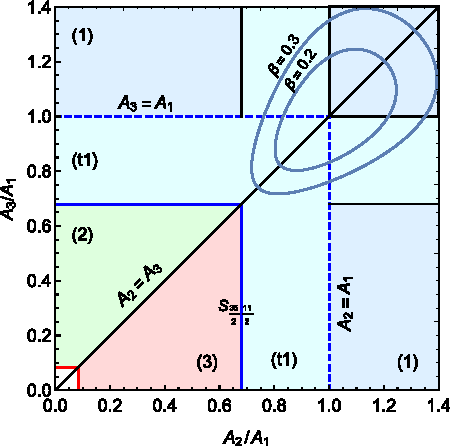
\includegraphics[width=.8\linewidth]{figures/wobb-phase-independent}
	\caption{Фазовая диаграмма качающейся моды для независимых жестких 
	моментов инерции. Красным показаны качения с наклоном в плоскости 
	(1,3), зеленым -- в плоскости (1,2), синим -- продольные качения, 
	голубым -- перпендикулярные, а белым -- недоступная область. Для 
	вычисления $\SJj$ выбраны значения $J = 35/2$, $j = 11/2$. Контуром 
	показана доступная область параметров при параметризации 
	$\mathcal{J}_k^\mathrm{rig} = \mathcal{J}_0^\mathrm{rig} \left(1 
	- \beta\sqrt{5/4\pi}\cos(\gamma_\mathrm{rig} - 2\pi k /3)\right)$.}
	\label{fig:independent}
\end{figure}% }}}
\begin{figure}% {{{
	\centering
	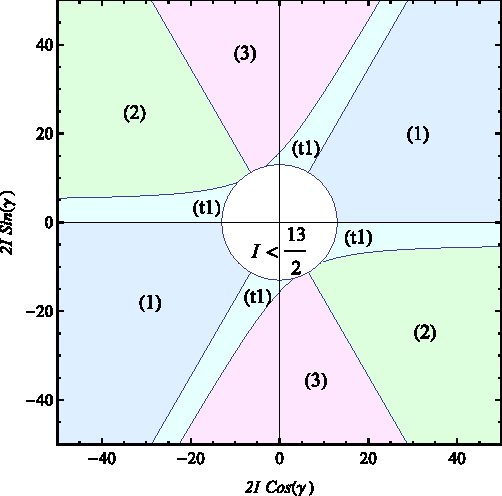
\includegraphics[width=.8\linewidth]{figures/wobb-phase-hydrodynamic}
	\caption{Фазовая диаграмма качающейся моды в гидродинамической модели 
	$\mathcal{J}_k = \tfrac{4}{3} \mathcal{J}_0 \sin^2(\gamma 
	- \tfrac{2}{3}k\pi) $. Красным показаны качения с наклоном в плоскости 
	(1,3), зеленым -- в плоскости (1,2), синим -- продольные качения, 
	голубым -- перпендикулярные, а белым -- недоступная область.}
	\label{fig:hydrodyn}
\end{figure}% }}}

Аналогичная ситуация наблюдается и для гидродинамической модели. 
Сначала, для малых значений $J$, моды качения отсутствуют вовсе. По мере 
возрастания $J$ ядро попадает в область продольных или перпендикулярных 
качений, а при дальнейшем увеличении орбитального момента, если параметр 
деформации $\gamma$ оказывается в определенных (широких) интервалах, ось 
вращения ядра наклоняется. Переход к наклонной оси вращения 
характеризуется достижением нуля частоты соответствующих качений 
и пересечением сепаратрисы. Зависимость частоты от орбитального момента 
показана на рисунке~\ref{fig:transition}.

\begin{figure}% {{{
	\centering
	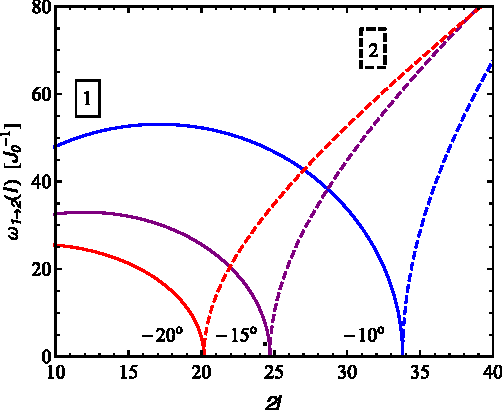
\includegraphics[width=.8\linewidth]{figures/wobb-tilted-transition}
	\caption{Зависимость частоты моды качений от орбитального момента ядра 
	и переход к вращению относительно наклонной оси для трех значений 
	параметра асимметрии $\gamma$.}
	\label{fig:transition}
\end{figure}% }}}
\begin{figure}% {{{
	\centering
	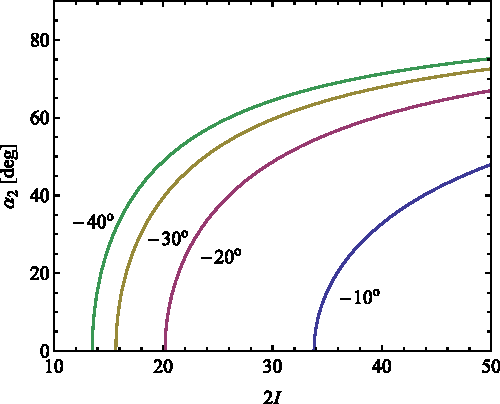
\includegraphics[width=.8\linewidth]{figures/tilted-alpha-evolution}
	\caption{Зависимость угла наклона оси вращения от орбитального момента 
	ядра для четырех значений параметра асимметрии $\gamma$.}
	\label{fig:alpha-evo}
\end{figure}% }}}

Необходимо заметить, что величина угла наклона оси вращения также 
зависит от орбитального момента. Это очевидно, если вспомнить выражения 
для $\cos\alpha_{2,3}$. Эволюция угла наклона для нескольких форм ядер 
представлена на рисунке~\ref{fig:alpha-evo}. Для асимптотически больших 
значений $J$ вращение происходит вокруг оси, перпендикулярной исходной 
оси 1, но из рисунка~\ref{fig:alpha-evo} видно, что угол наклона скорее 
выходит на медленно растущее плато. Чем сильнее ядро деформировано, тем 
быстрее возрастает и выходит на насыщение угол наклона при открытии 
соответствующей моды.

Касательно ядра \Pr{}, изложенный подход позволяет описать его yrast 
и качающуюся линии при использовании двух независимых параметров 
моментов инерции для ротационной моды и качающихся 
вращений~\cite{tilted-wobb}. Yrast серия соответствует $n=0$, 
а качающаяся -- $n=1$. Теоретические и экспериментальные данные по 
энергиям возбуждения приведены на рисунке~\ref{fig:th-exp}. Как видно, 
достигается хорошее согласие даже в интервале между $J = 27/2$ и $33/2$, 
где происходит переход к наклонной оси. Полученные таким образом 
параметры ядра равны
$\mathcal{J}^R_0 = 30.96$~МэВ$^{-1}$,
$\mathcal{J}^W_0 = 65.93$~МэВ$^{-1}$,
$\gamma = - 11.18$\textdegree,
а углы наклона оси вращения оказываются $\alpha_2=4.22$\textdegree, 
20.78\textdegree и 28.36\textdegree для J = $\tfrac{31}{2}$, 
$\tfrac{33}{2}$ и $\tfrac{35}{2}$, соответственно.

\begin{figure}% {{{
	\centering
	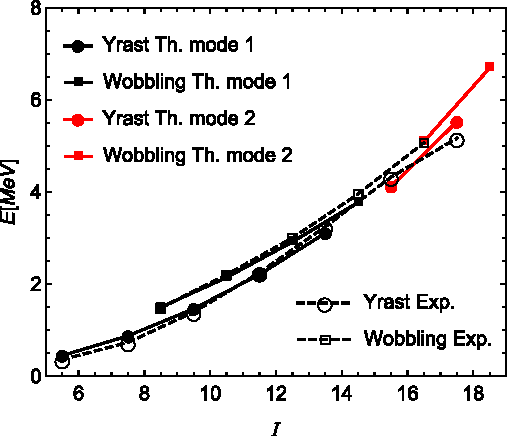
\includegraphics[width=\linewidth]{figures/yrast-wobb-th-exp}
	\caption{Сравнение экспериментальных~\cite{Pr2} и теоретических 
	энергий возбуждения yrast серии и качающейся моды.}
	\label{fig:th-exp}
\end{figure}% }}}

% }}}

\section{Заключение}% {{{

Ядра, не имеющие аксиальной симметрии, хотя и довольно редко, но 
встречаются в эксперименте и поддаются достаточно точному теоретическому 
описанию. Нахождение спектра трехосного ротора требует использования 
квазиклассического подхода, но даже с этим ограничением авторам удается 
достичь хорошего согласия с экспериментом.

Поиск трехосных ядер в эксперименте осуществляется в основном путем 
идентификации качающейся моды, которая служит прямым доказательством 
асимметричности ядра. Однако это не является единственным методом, 
и физики пытаются использовать другие способы идентификации таких форм.

Прерогативой аксиально асимметричных ядер также оказывается возможность 
вращения вокруг наклонной оси, в частности, не принадлежащей ни одной из 
главных плоскостей собственной системы координат эллипсоида инерции. 
Такие вращения имеют ряд занимательных свойств как, например, поворот 
оси вращения при изменении величины углового момента. Также интересен 
и переход от моды качения к наклонной оси при наличии неспаренного 
нуклона в ядре.

Дальнейшее изучение этой темы необходимо как с теоретической, так 
и с экспериментальной сторон, причем успехи теории особенно желательны 
при описании вероятностей электромагнитных переходов в сериях 
с наклонной осью вращения.

% }}}

\begin{thebibliography}{9}% {{{
	\bibitem{gs1}
		T.~R.~Werner and J.~Dudek,
		\href {https://doi.org/10.1006/adnd.1995.1001}
		{At. Data Nucl. Data Tables \textbf{59}, 1 (1995)}.

	\bibitem{gs2}
		P.~Möller, R.~Bengtsson, B.~G.~Carlsson, P.~Olivius, and T.~Ichikawa,
		\href{https://doi.org/10.1103/PhysRevLett.97.162502}
		{Phys. Rev. Lett. \textbf{97}, 162502 (2006)}.

	\bibitem{gs3}
		P.~Möller \textit{et al.},
		\href{https://doi.org/10.1016/j.adt.2008.05.002}
		{At. Data Nucl. Data Tables \textbf{94}, 758 (2008)}.

		
	\bibitem{gamma-rigid}
		P.~Buganu and R.~Budaca,
		\href{https://doi.org/10.1103/PhysRevC.91.014306}
		{Phys. Rev. C \textbf{91}, 014306 (2015)}.

	\bibitem{first-use}
		A. S. Davydov and G. F. Filippov,
		\href{https://doi.org/10.1016/0029-5582(58)90153-6}
		{Nucl. Phys. \textbf{8}, 237 (1958)}.


	\bibitem{Pr1}
		R. Garg \textit{et al.},
		\href{https://doi.org/10.1103/PhysRevC.92.054325}
		{Phys. Rev. C \textbf{92}, 054325 (2015)}.

	\bibitem{Pr2}
		J. T. Matta \textit{et al}.
		\href{https://doi.org/10.1103/PhysRevLett.114.082501}
		{Phys. Rev. Lett. \textbf{114}, 082501 (2015)}.

	\bibitem{tilted-wobb}
		R. Budaca,
		\href{https://doi.org/10.1103/PhysRevC.97.024302}
		{Phys. Rev. C \textbf{97}, 024302 (2018)}.


	\bibitem{overview}
		A. A. Raduta,
		\href{https://doi.org/10.1016/j.ppnp.2016.05.002}
		{Progr. Part. Nucl. Phys. \textbf{90}, 241–298 (2016)}.

\end{thebibliography}% }}}

\end{document}
